% \documentclass[aspectratio=169,notes]{beamer}
\documentclass[aspectratio=169]{beamer}
\usetheme[faculty=phil]{fibeamer}
\usepackage{polyglossia}
\setmainlanguage{english} %% main locale instead of `english`, you
%% can typeset the presentation in either Czech or Slovak,
%% respectively.
\setotherlanguages{russian} %% The additional keys allow
%%
%%   \begin{otherlanguage}{czech}   ... \end{otherlanguage}
%%   \begin{otherlanguage}{slovak}  ... \end{otherlanguage}
%%
%% These macros specify information about the presentation
\title[Artificial Intelligence Software (AIS)]{Artificial Intelligence Software, Lecture 2} %% that will be typeset on the
\subtitle{Introduction to VibeCoding 
\\ \ \\ \  } %% title page.
\author{Oleg Bulichev}
%% These additional packages are used within the document:
\usepackage{ragged2e}  % `\justifying` text
\usepackage{booktabs}  % Tables
\usepackage{tabularx}
\usepackage{tikz}      % Diagrams
\usetikzlibrary{calc, shapes, backgrounds}
\usetikzlibrary{decorations.pathreplacing,calligraphy,calc,graphs}
\usepackage{amsmath, amssymb}
\usepackage{url}       % `\url`s
\usepackage{listings}  % Code listings
\usepackage{subfigure}
% \usepackage{floatrow}
% \usepackage{subcaption}
\usepackage{mathtools}
\usepackage{todonotes}
\usepackage{fontspec}
\usepackage{multicol}
\usepackage{pdfpages}
\usepackage{wrapfig}
\usepackage{qrcode}
\usepackage{animate}
\usepackage{booktabs}
\usepackage{multirow}
\usepackage{graphicx}
\usepackage{colortbl}

\graphicspath{{resources/}}
\frenchspacing

\setbeamertemplate{caption}{\raggedright\insertcaption\par}
\usetikzlibrary{graphs}

% \usepackage[backend=biber,style=ieee,autocite=footnote]{biblatex}
% \addbibresource{biblio.bib}
% \DefineBibliographyStrings{english}{%
%   bibliography = {References},}

\newcommand{\oleg}[2][] {\todo[color=red, #1] {OLEG:\\ #2}}
\newcommand{\fbckg}[1]{\usebackgroundtemplate{\includegraphics[width=\paperwidth]{#1}}}%frame background

\usepackage[framemethod=TikZ]{mdframed}
\newcommand{\dbox}[1]{
\begin{mdframed}[roundcorner=3pt, backgroundcolor=yellow, linewidth=0]
\vspace{1mm}
{#1}
\vspace{1mm}
\end{mdframed}
}

\begin{document}
\setlength{\abovedisplayskip}{0pt}
\setlength{\belowdisplayskip}{0pt}
\setlength{\abovedisplayshortskip}{0pt}
\setlength{\belowdisplayshortskip}{0pt}

\fbckg{fibeamer/figs/title_page.png}
\frame[c]{\setcounter{framenumber}{0}
    \usebeamerfont{title}%
    \usebeamercolor[fg]{title}%
    \begin{minipage}[b][6.5\baselineskip][b]{\textwidth}%
        \textcolor{black}{\raggedright\inserttitle}
    \end{minipage}
    % \vskip-1.5\baselineskip

    \usebeamerfont{subtitle}%
    \usebeamercolor[fg]{framesubtitle}%
    \begin{minipage}[b][3\baselineskip][b]{\textwidth}
        \raggedright%
        \insertsubtitle%
    \end{minipage}
    \vskip.25\baselineskip
}
%   \frame[c]{\maketitle}

\fbckg{fibeamer/figs/common.png}

\note{\scriptsize \begin{itemize}
        \item \
    \end{itemize}}


\section{Why do we need an AI Assistant?}

\begin{frame}[t]{Concept: Exoskeleton for the Mind}
    \vspace*{-0.5cm}
    \begin{itemize}
        \item \textbf{Reducing Cognitive Load:} No need to memorize all syntax or CLI parameters.
        \item \textbf{Accelerating Routine:} Automating what you already know but do slowly.
        \item \textbf{Focus on Essence:} Shifting from "how to write" to "what to write".
    \end{itemize}
    \begin{figure}[H]
        \centering
\includegraphics[height=4cm,width=1\textwidth,keepaspectratio]{auf.jpeg}
            \vspace*{-0.3cm}
        \caption{\textit{"AI will not replace programmers, but programmers with AI will replace those without it."}}
        \label{fig:auf.jpeg}
    \end{figure}

\end{frame}

\begin{frame}[t]{Practical Use Cases}
    \begin{block}{Boilerplate Generation}
        \begin{itemize}
            \item Infrastructure: Docker Compose, Ansible playbooks.
            \item Data Mappers.
        \end{itemize}
    \end{block}
    \begin{block}{Complex Syntax}
        \begin{itemize}
            \item Regular Expressions (Regex).
            \item Complex SQL queries (Window functions, CTEs).
            \item Bash scripts and awk/sed magic.
        \end{itemize}
    \end{block}
\end{frame}

\begin{frame}[t]{Prototyping}
    \begin{itemize}
        \item Testing hypotheses in 5 minutes instead of an hour.
        \item Rapid MVP creation for idea validation.
        \item Translating code from one language to another (e.g., Python $\to$ C++).
    \end{itemize}
    \vspace{0.5cm}
    \alert{Important:} Prototype $\neq$ Production Code. But the path to it becomes shorter.
\end{frame}

\begin{frame}[t]{Reference Materials}
    \begin{itemize}
        \item \href{https://github.blog/news-insights/research/the-economic-impact-of-the-ai-powered-developer-lifecycle-and-lessons-from-github-copilot/}{[ENG] Github Copilot: Impact on developer productivity}
    \end{itemize}
    

\end{frame}

\section{How LLMs Work (Under the Hood)}

\begin{frame}[t]{LLM as a Prediction Engine}
    An LLM is not a database of facts, but a probabilistic distribution over the next token.
    $$ P(token_{t+1} | token_1, ..., token_t) $$
    \begin{itemize}
        \item \textbf{Token:} A piece of word (e.g., "ing", "the", " import"). ~0.75 words.
        \item The model assigns a probability to every possible next token.
        \item \textbf{Inference:} We sample from this distribution to generate text.
    \end{itemize}
\end{frame}

\begin{frame}[t]{Sampling Parameters: Temperature}
    \textbf{Temperature ($T$):} Controls the "creativity" (randomness) of the model.
    \begin{itemize}
        \item \textbf{Low $T$ ($0.1 - 0.3$):} Peaked distribution. Selects the most probable tokens.
        \begin{itemize}
            \item \textit{Use for:} Coding, Math, formatting JSON.
        \end{itemize}
        \item \textbf{High $T$ ($0.7 - 1.2$):} Flatter distribution. Allows less probable tokens.
        \begin{itemize}
            \item \textit{Use for:} Brainstorming, Storytelling, Creative writing.
        \end{itemize}
    \end{itemize}
    \href{https://youtube.com/shorts/XsLK3tPy9SI?si=JXLzts8JGzqE6Tr5}{[ENG] Temperature in action (Video)}
\end{frame}

\begin{frame}[t]{Sampling Parameters: Top-k \& Top-p}
    Strategies to avoid "garbage" tokens from the long tail.
    \begin{columns}[T]
        \begin{column}{0.48\textwidth}
            \textbf{Top-k:}
            \begin{itemize}
                \item Limits choices to the top $K$ most likely tokens (e.g., $K=50$).
                \item Hard cutoff.
            \end{itemize}
        \end{column}
        \begin{column}{0.48\textwidth}
            \textbf{Top-p (Nucleus):}
            \begin{itemize}
                \item Selects smallest set of tokens whose cumulative probability exceeds $P$ (e.g., $P=0.9$).
                \item Dynamic cutoff (adapts to confidence).
            \end{itemize}
        \end{column}
    \end{columns}
    \href{https://youtu.be/aDmp2Uim0zQ?si=teTTcRsDLtA3BuUH}{Top-k video}
\end{frame}

\begin{frame}[t]{Why Hallucinations Occur?}
    \begin{block}{Stochastic Nature}
        The model completes a \textit{pattern}, not retrieves a \textit{fact}.
        If the most statistically probable completion for "Library for X" is "X-Lib-Pro" (which doesn't exist), the model generates it.
    \end{block}
    \begin{alertblock}{Danger Zone}
        When the model doesn't know the answer, it "dreams" up a plausible-sounding one to satisfy the pattern of a helpful assistant.
    \end{alertblock}
\end{frame}

\section{Levels of Vibe Coding}

\begin{frame}[t]{Evolution of Interaction}
    From simple copy-paste to autonomous agents.
    \begin{enumerate}
        \item \textbf{Chat-based:} Manual context, Copy-Paste.
        \item \textbf{Inline / Autocomplete:} "Flow" in the editor.
        \item \textbf{Context-Aware:} Understanding the whole project.
        \item \textbf{Agentic:} Turnkey task execution.
    \end{enumerate}
\end{frame}

\begin{frame}[t]{Level 1-2: Chat and Autocomplete}
    \begin{block}{Level 1: Chat (ChatGPT Web)}
        \begin{itemize}
            \item Pros: Access to the smartest model.
            \item Cons: No project context, manual copying.
        \end{itemize}
    \end{block}
    \begin{block}{Level 2: Inline (Copilot Ghost Text)}
        \begin{itemize}
            \item Pros: Does not break the flow (Flow state). FIM (Fill-In-Middle).
            \item Cons: Works only in local context (current file).
        \end{itemize}
    \end{block}
\end{frame}

\begin{frame}[t]{Level 3-4: Agents}
    \begin{block}{Level 3: @Workspace Chat}
        \begin{itemize}
            \item RAG over the project. "Where is this class defined?", "How are these modules connected?".
        \end{itemize}
    \end{block}
    \begin{block}{Level 4: Agentic (Cursor Composer / Windsurf)}
        \begin{itemize}
            \item "Make frontend for our trained model".
            \item AI opens files, edits, runs terminal commands itself.
        \end{itemize}
    \end{block}
\end{frame}

\begin{frame}[t]{Hierarchy (Visual)}
    \begin{figure}
        \centering
        \begin{tikzpicture}
            \coordinate (A) at (-3,0);
            \coordinate (B) at (3,0);
            \coordinate (C) at (0,4);
            \draw[thick, fill=blue!10] (A) -- (B) -- (C) -- cycle;
            
            \draw[thick] (-2.25,1) -- (2.25,1);
            \draw[thick] (-1.5,2) -- (1.5,2);
            \draw[thick] (-0.75,3) -- (0.75,3);
            
            \node at (0,0.5) {Level 1};
            \node at (0,1.5) {Level 2};
            \node at (0,2.5) {Level 3};
            \node at (0,3.4) {Level 4};

            \node[right, anchor=west] at (3.5,0.5) {\textbf{Chat} (Copy-Paste)};
            \draw[dotted, thick] (2.4,0.5) -- (3.4,0.5);

            \node[right, anchor=west] at (3.5,1.5) {\textbf{Inline} (Copilot)};
            \draw[dotted, thick] (1.6,1.5) -- (3.4,1.5);
            
            \node[right, anchor=west] at (3.5,2.5) {\textbf{Context-Aware}};
            \draw[dotted, thick] (0.8,2.5) -- (3.4,2.5);
            
            \node[right, anchor=west] at (3.5,3.4) {\textbf{Agents}};
            \draw[dotted, thick] (0.2,3.4) -- (3.4,3.4);
        \end{tikzpicture}
        \caption{Pyramid of AI Autonomy in Development}
    \end{figure}
\end{frame}


\section{Dos and Don'ts}

\begin{frame}[t]{Task Separation}
    \begin{itemize}
        \item \textbf{High variability, low risk:} Ideal for AI.
        \item \textbf{Low variability, high risk:} Requires careful control.
    \end{itemize}
    Not all tasks are equally beneficial to delegate to AI. Blind trust leads to "future technical debt".
\end{frame}

\begin{frame}[t]{Green Zone (YES) - ML/Robotics}
    \begin{itemize}
        \item \textbf{Data Preprocessing:} Pandas/Numpy pipelines, data augmentation scripts.
        \item \textbf{Model Boilerplate:} Standard PyTorch/TensorFlow training loops, DataLoaders.
        \item \textbf{Visualization:} Matplotlib/Seaborn plots for EDA and metrics.
        \item \textbf{Infrastructure:} Dockerfiles for CUDA envs, ROS launch files/URDFs.
        \item \textbf{Documentation:} Explaining model architectures and math formulas.
    \end{itemize}
\end{frame}

\begin{frame}[t]{Red Zone (NO/Caution) - ML/Robotics}
    \begin{itemize}
        \item \textbf{Novel Architectures:} Designing SOTA models without understanding (hallucinated layers).
        \item \textbf{Safety-Critical Control:} Robot kinematics/dynamics where errors cause physical damage.
        \item \textbf{Subtle Math Errors:} Tensor dimension mismatches, incorrect gradients in custom loss functions.
        \item \textbf{Proprietary Data:} Never paste private datasets or patient data into the prompt.
    \end{itemize}
\end{frame}


\section{Impact on Qualification & Methodologies}

\begin{frame}[t]{Multiplier Effect}
    AI acts as a multiplier of your current qualification.
    $$ Result = Skill \times AI\_Factor $$
    \begin{itemize}
        \item Senior ($10 \times 1.5 = 15$): Acceleration, focus on architecture.
        \item Junior ($2 \times 1.5 = 3$): Help in learning, but risk of "illusion of knowledge".
        \item Zero ($0 \times 1.5 = 0$): Without a base, AI is useless for serious tasks.
    \end{itemize}
\end{frame}

\begin{frame}[t]{Methodology 1: TDD + AI (Synergy)}
    \textbf{Test Driven Development:}
    \begin{columns}[T,onlytextwidth]
        \begin{column}{0.49\textwidth}
        \begin{enumerate}
        \item You write a test (behavior specification).
        \item Test fails (Red).
        \item AI writes implementation to pass the test (Green).
        \item You refactor code with AI (Refactor).
    \end{enumerate}
    \textit{Example:} "Write a test for a function that IOUs (Intersection over Union) of two bounding boxes."
        \end{column}
        \begin{column}{0.49\textwidth}
            \vspace*{-1cm}
                \begin{figure}
        \centering
        \begin{tikzpicture}[scale=0.8]
            \node[draw, circle, red, thick] (R) at (0,2) {Red};
            \node[draw, circle, green!70!black, thick] (G) at (2.5,-1) {Green};
            \node[draw, circle, blue, thick] (Ref) at (-2.5,-1) {Refactor};
            
            \draw[->, thick, bend left] (R) to node[midway, right] {AI Code} (G);
            \draw[->, thick, bend left] (G) to node[midway, below] {Clean Up} (Ref);
            \draw[->, thick, bend left] (Ref) to node[midway, left] {New Test} (R);
        \end{tikzpicture}
        \caption{TDD Cycle}
    \end{figure}
        \end{column}
    \end{columns}
\end{frame}

\begin{frame}[t]{Methodology 2: BDD \& RDD (Specification-Driven Development)}
    \begin{block}{Behavior Driven Development (BDD)}
        \textbf{Concept:} Describe scenarios in plain language.
        \\ \textit{Example:} "Given a loaded YOLOv8 model, When input is a black image, Then 0 objects should be detected."
        \\ $\to$ AI translates this into `pytest-bdd` code effortlessly.
    \end{block}
    \begin{block}{Readme Driven Development (RDD)}
        \textbf{Concept:} Write the `README.md` with usage examples first.
        \\ AI uses the Readme as a specification to implement the internal logic (API, CLI arguments).
    \end{block}
\end{frame}

\begin{frame}[t]{Methodology 3: Type-First Design}
    \textbf{Idea:} Define complex types and interfaces before logic.
    \begin{itemize}
        \item Use Pydantic/Dataclasses to define schemas (e.g., `ModelConfig`, `InferenceResult`).
        \item AI is excellent at "filling in the blanks" if the types are strict.
        \item \textit{Robotics:} Define `Translation3d` and `Rotation3d` types, let AI write the transformation logic.
    \end{itemize}
\end{frame}

\begin{frame}[t]{Skills to Boost Vibe Coding}
    To use AI effectively, shift focus from syntax to:
    \begin{itemize}
        \item \textbf{System Design:} Modular architecture (Clean Arch). AI can write the function, but you define where it lives.
        \item \textbf{Code Review:} You read 10x more code than before. Spotting subtle broadcasting errors in PyTorch is a key skill.
        \item \textbf{Property-Based Testing:} Description of properties: "The output probability distribution must always sum to 1.0". (Refs: `Hypothesis`).
    \end{itemize}
\end{frame}

\begin{frame}[t]{Property-Based Testing (Deep Dive)}
    \begin{block}{Concept}
        Instead of: \textit{"If we input X, we get Y"} \\
        You formulate: \textit{"For any valid input data, property Z must hold."}
    \end{block}
    
    \begin{itemize}
        \item \textbf{Example (Sorting):}
        \begin{itemize}
            \item \textit{Standard:} \texttt{sort([3,1,2]) == [1,2,3]}
            \item \textit{Property:} Output is sorted AND contains same elements as input.
        \end{itemize}
        \item \textbf{Why use it?}
        \begin{itemize}
            \item \textbf{Edge Cases:} Tools (like Hypothesis) automatically find hard-to-spot bugs (NaNs, empty lists).
            \item \textbf{AI Synergy:} AI implements the logic, you define the physics/math \textbf{invariants} (e.g., "Probability sum = 1.0").
        \end{itemize}
    \end{itemize}
\end{frame}

\begin{frame}[t]{Danger for Juniors}
    \begin{itemize}
        \item Skipping "Basics": If you don't write bubble sort by hand at least once, you won't understand algorithm complexity.
        \item "StackOverflow Effect" on Steroids: Copying code without understanding.
        \item Debugging Complexity: Alien code (even from AI) is harder to debug than your own.
    \end{itemize}
\end{frame}

\begin{frame}[t]{Reference Materials}
    \begin{itemize}
        \item \href{https://tidyfirst.substack.com/p/tdd-with-github-copilot}{[ENG] Kent Beck: TDD with GitHub Copilot}
        \item \href{https://hypothesis.readthedocs.io/en/latest/}{[ENG] Hypothesis: Property-based testing for Python}
        \item \href{https://tom.preston-werner.com/2010/08/23/readme-driven-development.html}{[ENG] Readme Driven Development}
        \item \href{https://youtu.be/3le-v1Pme44?si=8EUp8FMyfkamfjHT}{[ENG] Spec-Driven Development (Video)}
        \item Clean Code and Clean Architecture -- Robert C. Martin
    \end{itemize}
\end{frame}



\begin{frame}[t]{Garbage In, Garbage Out}
    The quality of the model's answer is directly proportional to the quality of context and prompt.
    \begin{itemize}
        \item Charity of Intent.
        \item Constraints.
        \item Output Format.
    \end{itemize}
\end{frame}

\begin{frame}[t]{Core Techniques}
    \begin{enumerate}
        \item \textbf{Role Playing:} "Act as a Senior Python Developer specialized in FastAPI..."
        \item \textbf{Chain-of-Thought:} "Think step by step. First, analyze the structure..."
        \item \textbf{Few-Shot Prompting:} "Here is an example of my code. Create a new function in the same style."
    \end{enumerate}
\end{frame}

\begin{frame}[t]{Iterativity}
    Don't try to get perfect code in one prompt.
    \begin{itemize}
        \item Step 1: Describe the solution plan.
        \item Step 2: Implement class structure.
        \item Step 3: Write methods.
        \item Step 4: Write tests for this.
    \end{itemize}
\end{frame}

\begin{frame}[t]{Reference Materials}
    \begin{itemize}
        \item \href{https://platform.openai.com/docs/guides/prompt-engineering}{[ENG] OpenAI Prompt Engineering Guide}
        \item \href{https://habr.com/ru/articles/901426/}{Как писать промпты от Google (перевод)}
    \end{itemize}
\end{frame}


\section{Model Context Protocol (MCP)}

\begin{frame}[t]{The Isolation Problem}
    LLMs are usually locked in a chat "room". They don't see your database, can't access Jira, can't read server logs in real-time.
    \textbf{MCP} is a USB port for AI models.

    \begin{figure}[H]
        \centering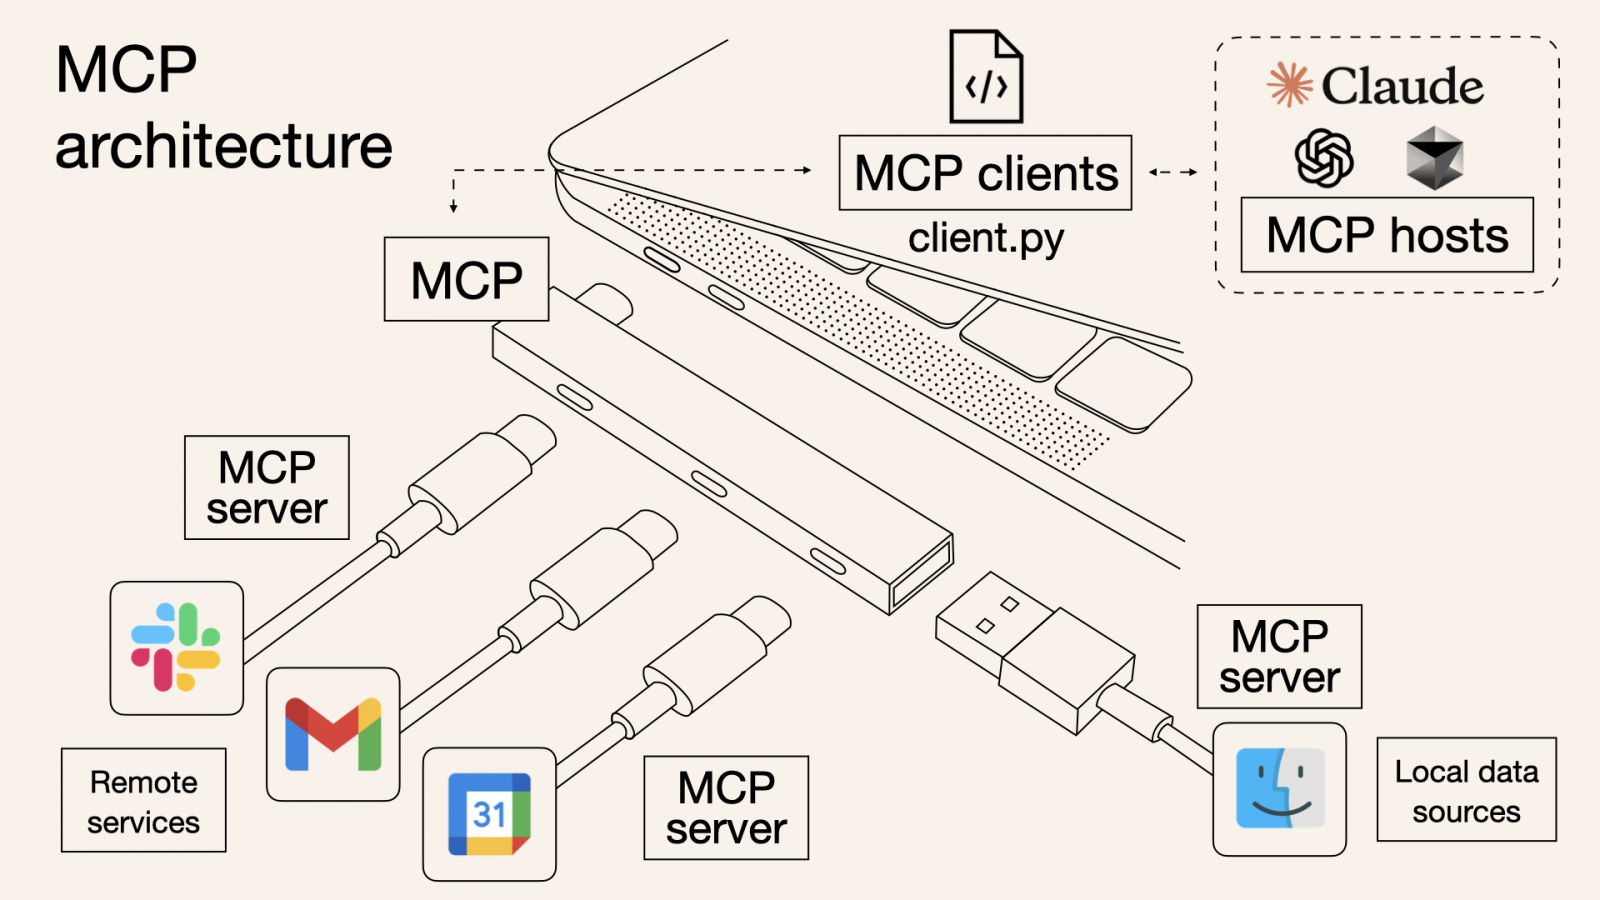
\includegraphics[height=4.5cm,width=1\textwidth,keepaspectratio]{mcp.jpg}
        % \caption{caption_name}
        \label{fig:mcp.jpg}
    \end{figure}
\end{frame}

\begin{frame}[t]{MCP Architecture}
    \begin{itemize}
        \item \textbf{MCP Host:} The application where you work (IDE: Cursor, Windsurf, Claude Desktop).
        \item \textbf{MCP Client:} Agent inside the host.
        \item \textbf{MCP Server:} Bridge to data (PostgreSQL, Google Drive, Local Filesystem).
    \end{itemize}
        \begin{figure}
        \centering
        \begin{tikzpicture}[node distance=2cm]
            \node[draw, rectangle] (Host) {Host (IDE)};
            \node[draw, rectangle, right of=Host, xshift=2cm] (Server) {MCP Server};
            \node[draw, cylinder, shape border rotate=90, right of=Server, xshift=1cm, aspect=0.25] (DB) {Data};
            
            \draw[<->, thick] (Host) -- node[above] {Protocol} (Server);
            \draw[<->, thick] (Server) -- (DB);
        \end{tikzpicture}
        \caption{MCP Connection Scheme}
    \end{figure}
\end{frame}



\begin{frame}[t]{Use Cases}
    \begin{itemize}
        \item "Check stock in Postgres DB and write an API endpoint".
        \item "Find requirements for this module in documentation on Google Drive".
        \item "Analyze error.log and propose a fix".
        \item "Open Blender, create a cube, and render it".
    \end{itemize}
\end{frame}

\begin{frame}[t]{Top Useful MCP Servers}
    \begin{itemize}
        \item \textbf{Context7 (Documentation):}
        \begin{itemize}
            \item Real-time access to docs for libraries (e.g., "How to use generic types in Pydantic v2?").
            \item Instead of hallucinating, the model searches valid documentation (RAG over the web).
        \end{itemize}
        \item \textbf{Puppeteer / Playwright (Browser Control):}
        \begin{itemize}
            \item Control a real browser: "Go to localhost:3000, login as admin, and take a screenshot."
            \item Essential for generating and debugging End-to-End (E2E) tests.
        \end{itemize}
        \item \textbf{Filesystem (Local Access):}
        \begin{itemize}
            \item Allows the agent to read logs (`/var/log/syslog`) or configs outside the project folder.
        \end{itemize}
    \end{itemize}
\end{frame}

\begin{frame}[t]{Reference Materials}
    \begin{itemize}
        \item \href{https://modelcontextprotocol.io}{[ENG] What does MCP means}
        \item \href{https://smithery.ai/}{[ENG] Smithery: MCP for everyone}
        \item \href{https://youtu.be/KnN3u1vugfA?si=GtnUHKdbaTUggaoJ}{Полный гайд по MCP (Видео)}
    \end{itemize}

\end{frame}


\section{Access and Payment from RF}

\begin{frame}[t]{Difficulties and Barriers}
    Most services (OpenAI, Anthropic, GitHub Copilot) require foreign cards and IP. Account bans.
    \begin{itemize}
        \item Obtain edu version of Github Copilot.
        \item \href{https://payment.mts.ru/tools/cursor}{[RUS] MTS Payment}
        \item Self-hosting (Ollama) as a workaround.
    \end{itemize}
\end{frame}

\begin{frame}[t]{Reference Materials}
    \begin{itemize}
        \item \href{https://youtu.be/i0CHdNl2vbA?si=w90Gj2mKFDCiz-eJ}{Ollama приложение}
        \item \href{https://youtu.be/91o27NsocR8?si=CLOur_UrM5fxqY-K}{Ollama cli}
    \end{itemize}
\end{frame}

\begin{frame}[t]{Best models}
    \framesubtitle{Video}
    \vspace{-0.6cm}
    \begin{figure}[H]
        \href{https://youtu.be/_i9UhGnOZCM?si=0OMvlfdiMjg9agub}{
            \centering
\includegraphics[height=6cm,width=1\textwidth,keepaspectratio]{best_vibe_coding.jpg}}
        \label{fig:best_vibe_coding.jpg}
    \end{figure}
\end{frame}

\begin{frame}[t]{Experimental Setup: Tools and Environment}
    \begin{itemize}
        \item \textbf{Development Environments:}
        \begin{itemize}
            \item \textbf{Cursor:} Used for 6 out of 9 models available out-of-the-box .
            \item \textbf{Cline:} Used for models requiring API integration via \textbf{Polza AI} aggregator .
        \end{itemize}
        \item \textbf{Model Selection:}
        \begin{itemize}
            \item \textbf{Anthropic:} Sonnet 4.5, Opus 4.5 .
            \item \textbf{Google:} Gemini 3 Pro, Gemini 3 Flash .
            \item \textbf{OpenAI:} GPT 5.2 (with \textit{Extra High Thinking} mode) .
            \item \textbf{Others:} Composer (Cursor), Kimi K2, GLM 4.7, Qwen 3 Max .
        \end{itemize}
    \end{itemize}
\end{frame}

\begin{frame}[t]{Methodology: The "Vibe Coding" Rules}
    \begin{itemize}
        \item \textbf{Initial Prompt:} Each model receives one comprehensive starting prompt describing the entire project.
        \item \textbf{Iterative Debugging:}
        \begin{itemize}
            \item If the output has issues, the model is allowed up to \textbf{5 additional calls} to fix bugs .
            \item Results are finalized after the 5th correction attempt.
        \end{itemize}
        \item \textbf{Evaluation Criteria:} Ability to build complex MVPs (Fantasy To-Do lists, Reddit scrapers, Admin dashboards, Video dubbing pipelines) from scratch.
    \end{itemize}
\end{frame}

\begin{frame}[t]{Key Findings: Best Performing Models}
    \begin{itemize}
        \item \textbf{GPT 5.2 (Overall Winner):}
        \begin{itemize}
            \item Won all tests decisively .
            \item Success is attributed to the \textbf{Extra High Thinking} mode, prioritizing reasoning time over speed .
        \end{itemize}
        \item \textbf{Claude Opus 4.5:}
        \begin{itemize}
            \item Exceptional logic and high-quality UI design .
            \item Performance is nearly on par with the leader, often working "perfectly" with minimal fixes .
        \end{itemize}
    \end{itemize}
\end{frame}

\begin{frame}[t]{Key Findings: Budget and Niche Solutions}
    \begin{itemize}
        \item \textbf{Gemini 3 Flash (Best Value):}
        \begin{itemize}
            \item Recognized as the best balanced choice for "budget AI coding".
            \item Offers a strong performance-to-cost ratio.
        \end{itemize}
        \item \textbf{Composer (Fastest):}
        \begin{itemize}
            \item The quickest model for small, specific tasks .
            \item Less effective for building entire systems from zero .
        \end{itemize}
    \end{itemize}
\end{frame}

\begin{frame}[t]{Final Conclusions}
    \begin{itemize}
        \item \textbf{Thinking vs. Result:} There is a clear correlation between the model's reasoning time and the quality of the final code .
        \item \textbf{Shift in Development:} The bottleneck in 2026 is no longer writing code, but \textbf{architecture planning, documentation study, and algorithm design}.
        \item \textbf{One-Prompt MVPs:} It is now viable to create fully functional startup MVPs with a single well-structured prompt.
    \end{itemize}
\end{frame}


\begin{frame}[t]{IDE-Based Tools}
    \begin{itemize}
        \item \textbf{Cursor (VS Code Fork)}
        \begin{itemize}
            \item \textbf{Pros:} Deep codebase understanding (200k context), background agents, multi-file editing.
            \item \textbf{Cons:} Steeper learning curve, recently changed pricing (removed unlimited plans).
        \end{itemize}
        \item \textbf{Windsurf (Codium)}
        \begin{itemize}
            \item \textbf{Pros:} "Flow-aware" development, excellent context management, fast response times.
            \item \textbf{Cons:} Credit-based usage can be confusing, some find completion slower than Cursor.
        \end{itemize}
    \end{itemize}
\end{frame}

\begin{frame}[t]{Official Ecosystems: Claude Code \& Copilot}
    \begin{itemize}
        \item \textbf{Claude Code (Anthropic CLI)}
        \begin{itemize}
            \item \textbf{Pros:} Most advanced logic (Sonnet 4.5/Opus 4.5), no hidden fees, "Thinking Mode".
            \item \textbf{Cons:} CLI-based (lack of GUI for some), can burn tokens quickly in complex tasks.
        \end{itemize}
        \item \textbf{GitHub Copilot (Microsoft)}
        \begin{itemize}
            \item \textbf{Pros:} Most affordable ($10/mo$), native VS Code integration, very stable.
            \item \textbf{Cons:} Agent mode can be slower/less powerful than specialized rivals.
        \end{itemize}
    \end{itemize}
\end{frame}

\begin{frame}[t]{Specialized Agents: Goose \& Cline}
    \begin{itemize}
        \item \textbf{Goose (Block/GitHub)}
        \begin{itemize}
            \item \textbf{Pros:} Open-source client, supports any model via OpenRouter/Local LLMs.
            \item \textbf{Cons:} Slower process, purely agentic (autonomous) approach might be harder to control.
        \end{itemize}
        \item \textbf{Cline (formerly Kodu)}
        \begin{itemize}
            \item \textbf{Pros:} Full transparency in costs, checkpointing (rollback feature), "Bring-Your-Own-Key" (BYOK).
            \item \textbf{Cons:} Requires manual API management, strictly agent-focused.
        \end{itemize}
    \end{itemize}
\end{frame}

\begin{frame}[t]{Comparison Summary}
    \begin{table}
        \footnotesize
        \centering
        % \rowcolors{2}{gray!10}{white} % Optional: if you want alternating colors
        \begin{tabularx}{\textwidth}{l X X}
        \toprule
        \textbf{Tool} & \textbf{Key Strength} & \textbf{Main Weakness} \\ 
        \midrule
        \textbf{Cursor} & Deep Context/Refactoring & Complex UI/Pricing \\ 
        \addlinespace
        \textbf{Claude Code} & Best Reasoning/Thinking & CLI-only interface \\ 
        \addlinespace
        \textbf{Windsurf} & Flow/UX Speed & High Credit Consumption \\ 
        \addlinespace
        \textbf{Copilot} & Affordability/Integration & Limited Agent Power \\ 
        \addlinespace
        \textbf{Bolt/V0} & Rapid Prototyping (Vibe) & Hard to maintain long-term \\ 
        \bottomrule
        \end{tabularx}
    \end{table}
\end{frame}

\begin{frame}[t]{Conclusions: The Shift to Agentic Coding}
    \begin{itemize}
        \item \textbf{From Assistant to Agent:} Tools now plan, run terminal commands, and debug themselves.
        \item \textbf{The Bottleneck:} Reasoning (Thinking) is now more important than raw speed for complex MVPs.
        \item \textbf{Educational Risk:} Over-reliance on agents might hinder learning fundamentals for beginners.
        \item \textbf{Best Strategy 2026:} Use Claude Code for logic, Cursor/Windsurf for codebase navigation, and Gemini Flash for budget tasks.
    \end{itemize}
\end{frame}

\begin{frame}[t]{Reference Materials}
    \begin{itemize}
        \item \href{https://youtu.be/6NK4Pona2fY?si=y2-4Sg8qcnjxAqsl}{Claude Code: полный гайд по AI-кодингу (хаки, техники и секреты)}
        \item \href{https://youtu.be/tCGju2JB5Fw?si=9tIEuLm6BGDu8_HB}{We Tier Ranked Every AI Coding Assistant}
        \item \href{https://youtu.be/uPc_WDD5HqU?si=W41o-Yy_HSF7HwOK}{Windsurf vs Copilot vs Cursor In 2026 (Pros, Cons, \& Pricing Update)} 
        \item \href{https://youtu.be/I88olg5UBEg?si=usMMU8-CiJ6juGsE}{ИИ Агент Для Программирования — КАК ВЫБРАТЬ? (Cursor, Windsurf, Goose, VS code, Cline…)}
    \end{itemize}
\end{frame}

\fbckg{fibeamer/figs/last_page.png}
\frame[plain]{}

\end{document}